\subsection{Case study: multi-camera \gls{lkas} sharing the platform with other applications}
\begin{figure}[t]
\centerline{
    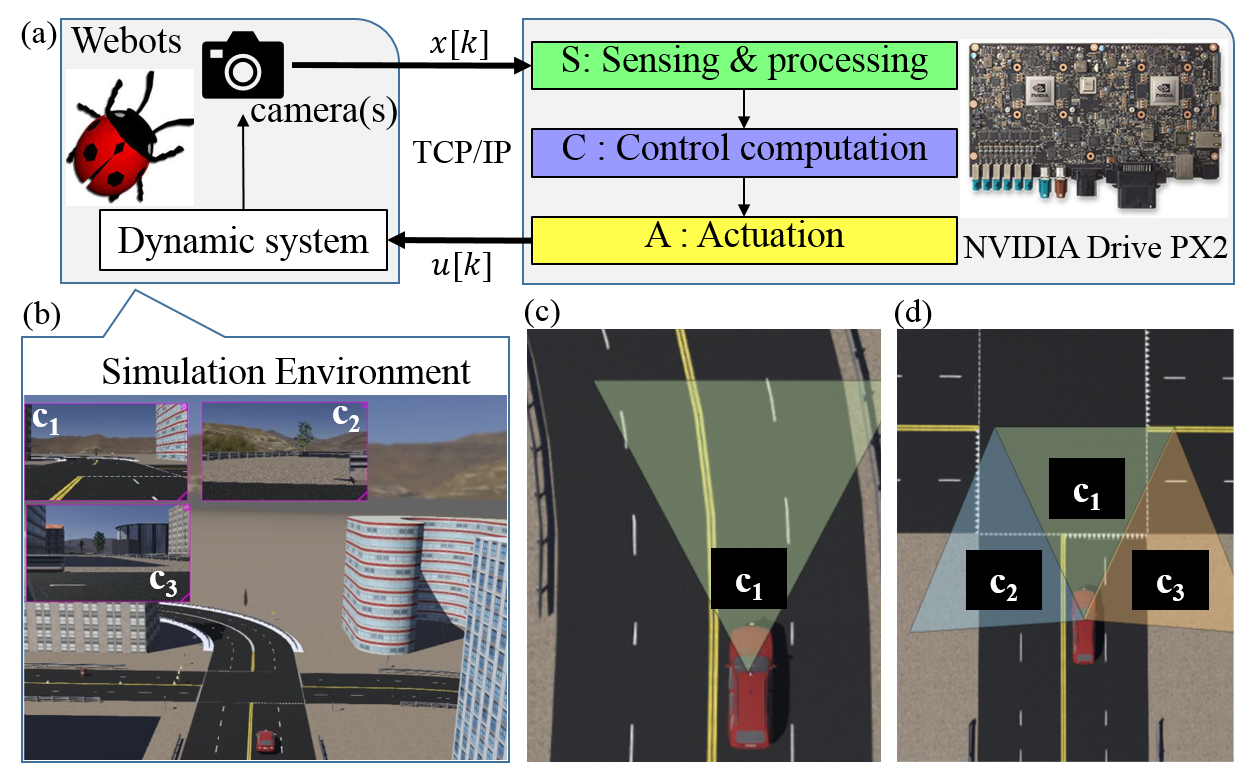
\includegraphics[scale=0.5]{images/HiL.png}
    }
    \caption{(a) \Gls{ibc} system block diagram and the \gls{hil} simulator. (b) a snapshot of the \gls{hil} simulation environment in webots. (c) \gls{lkas} using single camera. (d) multi-camera \gls{lkas}; $c_1$, $c_2$, $c_3$ are the cameras.}
    \label{fig:ch5_IBC_setting}
  %  \vspace{-2em}
\end{figure}
We consider a concrete case study of a multi-camera \gls{lkas}. The goal of the \gls{lkas} is to steer the vehicle autonomously to follow the center line of a lane. Multiple cameras are used since the field-of-view of a single camera is not sufficient to detect the lanes when the vehicle has to make sharp turns, e.g., at a T-junction. Fig.~\ref{fig:ch5_IBC_setting}(c) and (d) show the two different scenarios in the \gls{lkas} system. The first scenario $s_1$ (see Fig.~\ref{fig:ch5_IBC_setting}(c) occurs when the vehicle is navigating on a road with no sharp turns. In scenario $s_1$, only one camera $c_1$ needs to be active. The second scenario $s_2$ (see Fig.~\ref{fig:ch5_IBC_setting}(d) happens when the vehicle needs to take a sharp turn. In this case, all three cameras $c_1,\ c_2$ and $c_3$ need to be active. 
During runtime the scenarios are detected based on the following: i) when there is a lane detected by camera $c_1$ and there is no request to make a turn, the \gls{lkas} executes in scenario $s_1$; ii) when there is no lane detected by camera $c_1$ or there is a request to make a turn, the \gls{lkas} executes in scenario $s_2$. Our multi-camera \gls{lkas} is sharing the NVIDIA Drive PX2 platform with two other data-intensive applications - \gls{odt} and \gls{aeb}.

\subsection{\Gls{spade} input: \gls{ibc} application}
\subsubsection{Image sensing and processing ($\taskS$)}
The main stages in the compute-intensive image sensing and processing of an automotive \gls{ibc} system are the \gls{isp} pipeline, environment perception and application-specific rendering (if required) (shown in Fig.~\ref{fig:ch5_SandPP}(a)). The \gls{isp} pipeline is generic for all \gls{ibc} applications. Environment perception involves application-specific preprocessing, feature extraction and inference. Rendering refers to the display of relevant information on the dashboard or screen of the vehicle and is application-specific. Below, we explain these stages in detail for our \gls{lkas} system case study. 
\\[1ex]
\noindent\textbf{\Acrfull{isp} pipeline} 
The NVIDIA Drive PX2 comes with a Tegra configurable \gls{isp} hardware and supports different image types - CUDA, OpenGL, NvMedia - and different pixel formats - RAW, grayscale, RGB, Red Clear Clear Blue (RCCB), RGB alpha (RGBA),  YUV. NvMedia is an NVIDIA proprietary framework which uses dedicated hardware blocks on the Tegra \glspl{soc} for faster image processing.  Algorithmic analysis of a closed-source proprietary \gls{isp} pipeline is not possible. The stages common to generic \gls{isp} pipelines are explained in~\cite{buckler}.
For our \gls{lkas}, the \gls{gmsl} camera~\cite{nvidiadrive} captures the image frame at a fixed frame rate, 30 fps. Each frame then goes through the closed-source \gls{isp} pipeline to obtain an image in $\ll$NvMedia, YUV$\gg$ format. 
\\[1ex]
\noindent\textbf{Perception} 
The perception stage performs a set of application-specific preprocessing, feature extraction and control state computation steps on the image obtained from the \gls{isp}. 

The preprocessing step in \gls{lkas} (shown in Fig.~\ref{fig:ch5_SandPP}(a)) involves converting the image in $\ll$NvMedia, YUV$\gg$ format to the $\ll$CUDA, RGBA$\gg$ and $\ll$OpenGL, RGBA$\gg$ image type and pixel formats. Closed-source functions `image streamer' and `format conversion' from NVIDIA perform the image type conversions and pixel format conversions, respectively. The $\ll$CUDA, RGBA$\gg$ format is used for applications that use \glspl{gpu} and $\ll$OpenGL, RGBA$\gg$ for rendering.

The features to extract are application-specific. The \gls{lkas} extracts the lanes from the image using the NVIDIA proprietary (pre-trained) high-precision \gls{dnn} \textit{Lanenet}~\cite{wang2018lanenet} that enables pixel-level lane detection. 
Lanenet executes on the GPU and its input is a $\ll$CUDA, RGBA$\gg$ image. The output of Lanenet is the position values of all the lane containing pixels, i.e., a set of polyline values in the pixel domain.

Finally, the lateral deviation of the vehicle from the center of the lane is derived. A homography transformation matrix~\cite{hartley2003multiple} is computed at design time. This matrix is stored in the platform memory and is used at runtime to compute the position values of the detected polylines from Lanenet.
The left and right lane polylines are then fit to a second degree polynomial. For a given look-ahead distance,
the center of the lane is derived using these polynomials while the center of the image gives the vehicle`s current position. Using these, the lateral deviation is calculated at the look-ahead distance. The homography transformation at runtime needs to be done only for the identified lane pixels. 
\\[1ex]
\noindent\textbf{Rendering}
For \gls{lkas}, the rendered image consists of the pre-processed image captured by the camera in $\ll$OpenGL, RGBA$\gg$ format superimposed with the polylines detected by Lanenet. 
The rendering step is not important for the correct functioning of \gls{lkas}. 
Rendering is used for debugging and often provided as an add-on for automotive customers for visual pleasure. 
\begin{figure}[t]
    \centering
    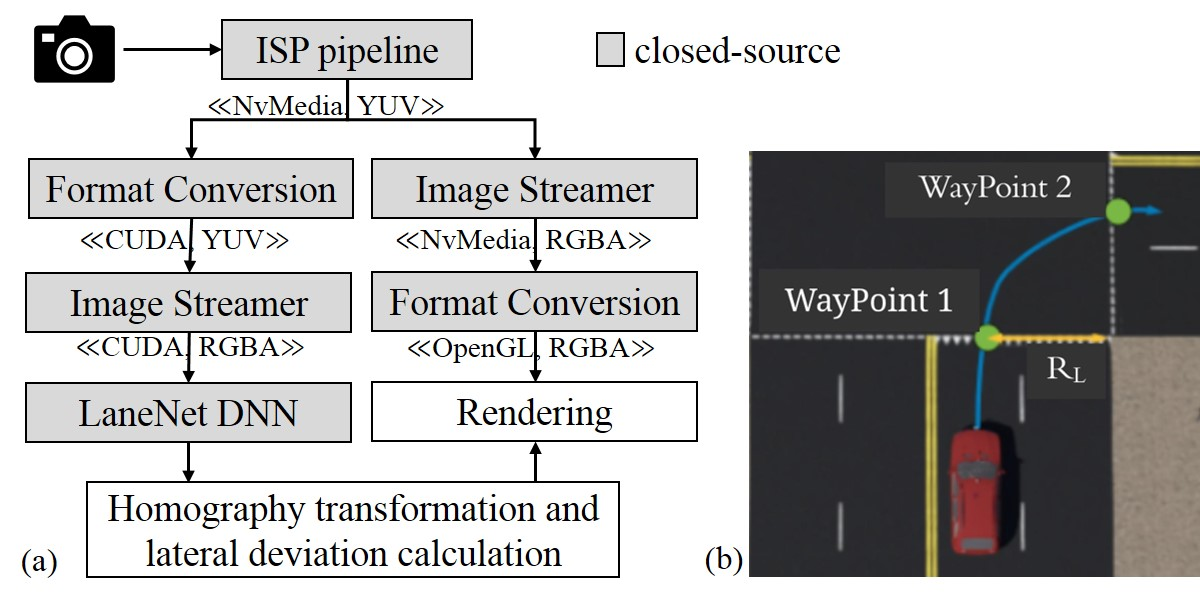
\includegraphics[scale=0.5]{images/SnPP.jpg}
    \caption{(a) The block diagram of image sensing and processing task $\taskS$. (b) Path planning for scenario $s_2$.}
    \label{fig:ch5_SandPP}
    %\vspace{-2em}
\end{figure}

\subsubsection{Control computation ($\taskC$) and actuation ($\taskA$) tasks} 
The default \textbf{scenario {s\textsubscript{1}}} 
persists when there is always a lane detected in the image captured by the camera $c_1$ and when there is no request to take a turn, e.g., at a junction. For this scenario, the \gls{lkas} controller explained in Section~\ref{sec:ch5_embeddedIBC} is used. 
\textbf{scenario {s\textsubscript{2}}} occurs when there is no lane detected by camera $c_1$ or when there is a request to take a sharp turn. Here the control computation is a standard path planning algorithm. The direction of the turn is user input or determined arbitrarily if lanes are detected on both $c_2$ and $c_3$. If no lanes are detected in any of the cameras, \gls{aeb} is activated.
Actuation task $\taskA$ actuates the vehicle steering to the desired value communicated to it by the control computation task.

\subsection{Formal modelling}
\begin{figure}[t]
    \centering
    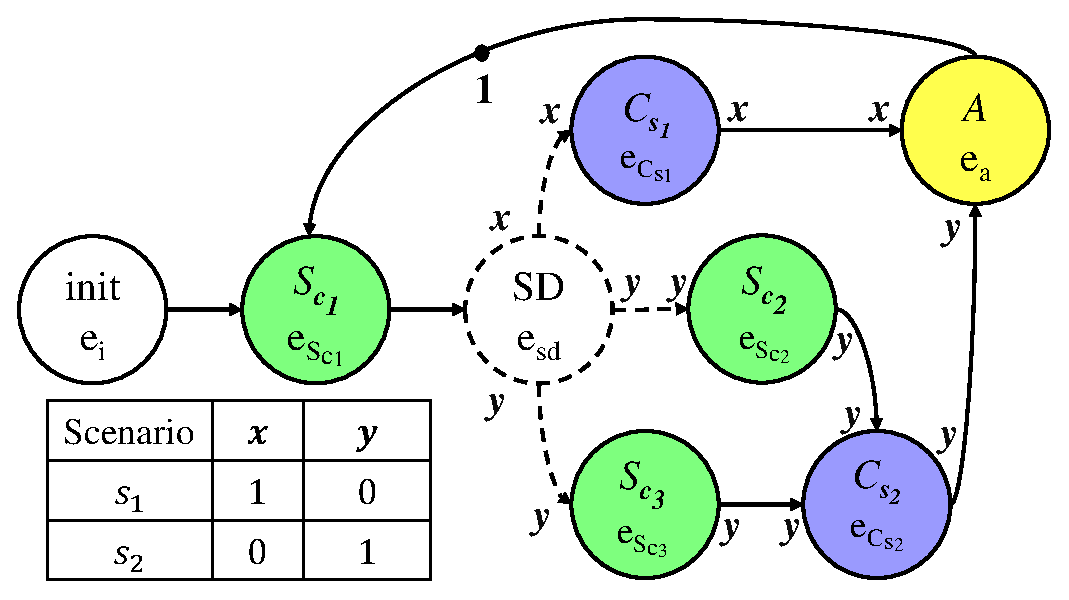
\includegraphics[scale=0.5]{images/sadf2.eps}
    \caption{Multi-camera \gls{lkas} \gls{sadf} model.}
    \label{fig:ch5_SADF2}
    %\vspace{-2em}
\end{figure}
The application is modelled as a dataflow graph (see Fig.~\ref{fig:ch5_SADF2} and Section~\ref{sec:ch5_MoC}). The applications sharing the platform act as load and the platform is modelled as a platform graph (see Fig.~\ref{fig:drive_platform}) using the available information~\cite{nvidiadrive} (see Section~\ref{sec:ch5_embeddedIBC}). 

The \gls{lkas} has two application scenarios. The \textit{init} actor models platform initialisation. The $\taskS_{c_1},\ \taskS_{c_2}$ and $\taskS_{c_3}$ actors model the image sensing and processing tasks for cameras $c_1,\ c_2$ and $c_3$. Each sensing task has the internal structure shown in Fig.~\ref{fig:ch5_SandPP}(a). $\taskC_{s_1}$ and $\taskC_{s_2}$ model the control computations for scenarios $s_1$ and $s_2$. 
The actuation task is modelled by actor $\taskA$. The scenario detector actor $SD$ determines which scenario the application runs in. $\actorET_i,\ \actorET_{\taskS_{c_1}},\ \actorET_{sd},\ \actorET_{\taskC_{s_1}},\ \actorET_{\taskS_{c_2}},\ \actorET_{\taskS_{c_3}},\ \actorET_{\taskC_{s_2}}$ and $\actorET_a$ are the execution times of the corresponding actors.

Note that the workload for this case is defined by the combination of application scenarios, non-predictable timing behaviour of the closed-source industrial platform and the platform load. Each platform load condition is abstracted as a variant (see Table~\ref{table:variants}) for a systematic analysis.
The parameters that change based on the workload are $x,\ y$ shown in Fig.~\ref{fig:ch5_SADF2} (due to the application scenarios) and the execution times of all actors (due to the platform load).

\subsection{Analysis and design}
\subsubsection{System mapping and mapping configurations}
The tasks/actors need to be mapped to the Tegra \gls{soc} resources - \gls{cpu}, \gls{igpu}, \gls{dgpu} and memory, where \gls{cpu} refers to the A57 and denver2 cores. Note that there are two Tegra \glspl{soc} in the NVIDIA Drive PX2 platform. The options available for the developer when mapping to the PX2 platform are limited. Priorities for tasks can only be assigned on \gls{cpu} resources. The tasks mapped to the \glspl{gpu} are executed by the proprietary NVIDIA scheduler and the execution times for such tasks vary the most due to the (unpredictable) scheduler~\cite{intro_nvidia_no_predict}. 

The mapping configuration does not include the schedule of tasks mapped to \glspl{gpu} as it is not controllable. Note that init, the homography computation step of $\taskS$, $SD$, $\taskC$ and $\taskA$ are always mapped to \glspl{cpu} and the other steps of $\taskS$ are always mapped to \glspl{gpu}. The \glspl{gpu} can only be accessed through the \glspl{cpu} in the same \gls{soc} by a blocking call.

\subsubsection{Profiling and timing analysis}
Platform-aware profiling is a crucial step in this instance of the \gls{spade} flow. 
Since there are closed-source functions in the application and a non-real-time Ubuntu \gls{os}, the \glspl{wcet} of tasks in the application are difficult to predict. The \gls{wcet} of tasks depends on three factors: scenario of the \gls{ibc} application, choice of mapping, and the load on the platform due to the shared applications. For our case study, we consider two other applications - \gls{odt} and \gls{aeb} - sharing the platform. Both applications take camera images as input. 

We define variants $v.i$ to characterise and abstract multiple workload scenarios for a structured profiling and timing analysis.
The definition of variants is not a necessity for the basic version of the \gls{spade} flow. However, it helps to classify the expected runtime scenarios and perform profiling and timing analysis in a structured way for the designer.
The variants we consider based on our mapping choice and platform load are defined in Table~\ref{table:variants}. 
The mapping is characterised based on mapping the \gls{lkas} application to the \gls{igpu} or the \gls{dgpu}, as preliminary experiments show that compute-intensive imaging tasks perform better on \glspl{gpu}. Tasks mapped to \glspl{cpu} take less than 5\% of the overall \gls{wcet} and are not explicitly considered.
The platform loads \gls{aeb} and \gls{odt} denote the mapping of these applications to the same \gls{gpu} as the \gls{lkas}. The platform load ODTs denotes the mapping of \gls{odt} and \gls{lkas} to multiple \glspl{gpu} (of the same type) so that there is task sharing between \glspl{gpu}. This can be done in the NVIDIA platform by assigning just the type of \gls{gpu} for the applications; then the proprietary scheduler allocates tasks between multiple \glspl{gpu}. This can be observed by analysing the \gls{gpu} utilisation (explained in Section~\ref{sec:ch5_HiL}).

Note that due to the closed-source \gls{gpu} scheduler of NVIDIA, the workload due to the application scenarios and the platform load conditions at runtime cannot be distinguished. 
Thus, the abstraction as variants is a means to enable the optimal system-scenario identification and runtime reconfiguration (explained in Section~\ref{sec:ch5_runtime_nvidia}). 

\begin{table}[t]
\caption{Characteristics of variants based on mapping choice and load conditions}
\scriptsize
\label{table:variants}
\vspace{-1em}
\centering
\begin{threeparttable}	
		\setlength\tabcolsep{1pt}
\begin{tabular}{|c|c|c|c|c|c|c|c|c|c|c|}
\hline
variants & v.1  & v.2  & v.3  & v.4  & v.5  & v.6  & v.7                                                & v.8                                                & v.9  & v.10 \\ \hline
mapping  & \gls{dgpu} & \gls{igpu} & \gls{dgpu} & \gls{igpu} & \gls{dgpu} & \gls{igpu} & \gls{dgpu}                                               & \gls{igpu}                                               & \gls{dgpu} & \gls{igpu} \\ \hline
load     & -    & -    & \gls{aeb}  & \gls{aeb}  & \gls{odt}  & \gls{odt}  & \begin{tabular}[c]{@{}c@{}}\gls{aeb},\\ \gls{odt}\end{tabular} & \begin{tabular}[c]{@{}c@{}}\gls{aeb},\\ \gls{odt}\end{tabular} & ODTs & ODTs \\ \hline
\end{tabular}
\begin{tablenotes}
			\footnotesize
			\item{ODTs: Object detection and tracking with task sharing between \glspl{gpu}} 
\end{tablenotes}
\end{threeparttable}
\end{table}

For profiling, a database of around 200 images (captured by the \gls{gmsl} camera) is identified with varying image workload. Considering image workload variations is important since they affect the \gls{wcet} analysis. The image for the minimal workload has no lane markings and no other vehicles on the road; for the maximal workload, it contains three lane markings and other vehicles. For each variant, each image from the database is run on the PX2 for 10000 iterations.

The worst-case sensor-to-actuator delay $\tau_{wc}$ and sampling period $h_{wc}$ are computed as explained in Section~\ref{sec:ch5_relation}. 
The execution times of each task are profiled over all the variants and the maximum value is taken as the estimated \gls{wcet} of the corresponding task.
This \gls{wcet} estimate is used in the application \gls{sadf} model. $\tau_{wc}$ and $h_{wc}$ are then computed. Note that though this worst-case rarely happens, it is needed to guarantee stability of the \gls{ibc} system.
Similarly, for each variant $v.i$, the third quartile values of the measured execution times of each task (profiled for the corresponding variant) is used to compute $\tau_i$ and $h_i$. We thus avoid the measured \glspl{wcet} for the majority of the analyzed workload scenarios to avoid overly pessimistic model predictions. 

\subsubsection{Controller design}\label{sec:ch5_control_Design_stability}
The controller for scenario s\textsubscript{1} is designed as explained in Section~\ref{sec:ch5_embeddedIBC}. 
The standard linear quadratic regulator control is used to design the state feedback gain $\Kgain_{i}$ and the feed forward gain $\Fgain_{i}$ for each variant $v_i$. 
The control configuration $\Configuration_{\workloadScenario}^c$ is then defined as a tuple $\Configuration_{\workloadScenario}^c = (\tau_{i}, h_{i}, \Kgain_{i}, \Fgain_{i})$. For each version, only $\Configuration_{\workloadScenario}^c$ needs to be stored in the memory during implementation. 
The stability of this switched system is analysed by deriving \glspl{lmi} that check for the existence of a \gls{cqlf} (see Section~\ref{sec:ch5_controller_stability}).

For scenario s\textsubscript{2}, the path planning algorithm identifies two waypoints once the direction to turn is determined (illustrated in Fig.~\ref{fig:ch5_SandPP}(b) for a 90 degree turn). Waypoint 1 is the centre of the lane from where the vehicle has to start turning and Waypoint 2 is the centre of the lane after the turn, from where we expect scenario $s_1$ (see Fig.~\ref{fig:ch5_SandPP}(b)). This can be predicted based on the turning radius $R_L$. The steering angle $\delta_f=atan\left(\frac{L_{wb}}{R_L}\right)$, where $L_{wb}$ is the wheelbase of the vehicle. This steering angle is constantly applied from Waypoint 1 until the vehicle reaches Waypoint 2 and then task $\taskS$ repeats. Only $L_{wb}$ needs to be stored in memory for scenario $s_2$.

\subsection{System-scenario identification, implementation and runtime reconfiguration mechanism}
\label{sec:ch5_runtime_nvidia}
The variants defined in this section classify the expected runtime scenarios (as explained in Table \ref{table:variants}). The variants are useful in the profiling and timing analysis step in the basic \gls{spade} flow. 
A system scenario abstracts multiple variants with the same sampling period and optimal system scenarios are identified as explained in Section~\ref{sec:ch5_ch5_sys_scenario}. 
During runtime, we keep track of the start and finishing time of $\taskS$, i.e., the sensing delay, to check for which system scenario we need to execute from the \gls{lut}.
The control and mapping configurations of the variants and their relation to system scenarios are stored as a \gls{lut} in platform memory for runtime implementation. 
After identifying the system scenario, we load the corresponding control configuration $\Configuration_{\workloadScenario}^c$ and execute $\taskC$.
The mapping configuration is then loaded for the subsequent arriving frame. 
Note that even though control configurations are loaded every frame, mapping configurations cannot be loaded until after the system scenario identification is completed and as such there is a delay in loading mapping configuration by one frame.
The classification as variants is thus essential in the identification of the system scenario at runtime 
as the scenario identification at runtime is dependent on the current mapping as well. 
An \gls{lqr} controller designed for the worst-case ($\tau_{wc},h_{wc}$) and its corresponding control configuration $\Configuration_{s_wc}^c$ is also stored in the memory as the worst-case system scenario.
At runtime, system scenarios are switching (as explained in Section~\ref{sec:ch5_control_Design_stability}) based on the load and/or mapping choices.